\chapter{Experiments and Evaluations\label{cha:chapter4}}

To evaluate the Frankenbot's modular architecture on the basis of the user experience, the surveys has been conducted. 
\\~\\
For accomplishment of this research, random users were selected irrespective of their profession, studies background and any race or gender discrimination. But the age limit constraint was set to be above 18. As participants were considered to be accused of a robbery and have to chat with a detective bot and answer his questions which can be a bit rude and straight forward for youngsters below 18. So the participant with the minimum age was 22. On contrary, the one with the maximum age was 34. And the average age calculated as 25.65 with the standard deviation of 2.37. Visuals have been shown in the Figure \ref{fig:ageGraph}.

\begin{figure}[!h]
    \centering
    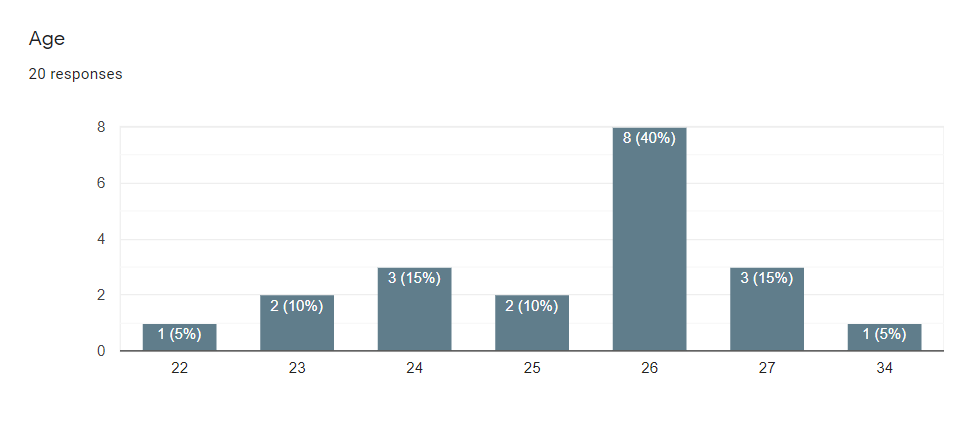
\includegraphics[width=0.9\textwidth]{img/Age_Graph.PNG}
    \caption{Age stats of participants}
    \label{fig:ageGraph}
\end{figure}
\\~\\
Total 20 users participated in this study. Most of them appeared to be from technical background as maximum of them were students from different universities. Secondly, majority of participants revealed themselves to be IT employees other than the students. While remaining revealed themselves as engineer, teacher and business qualified. More details have been shown in the Figure \ref{fig:profGraph}.

\begin{figure}[!h]
    \centering
    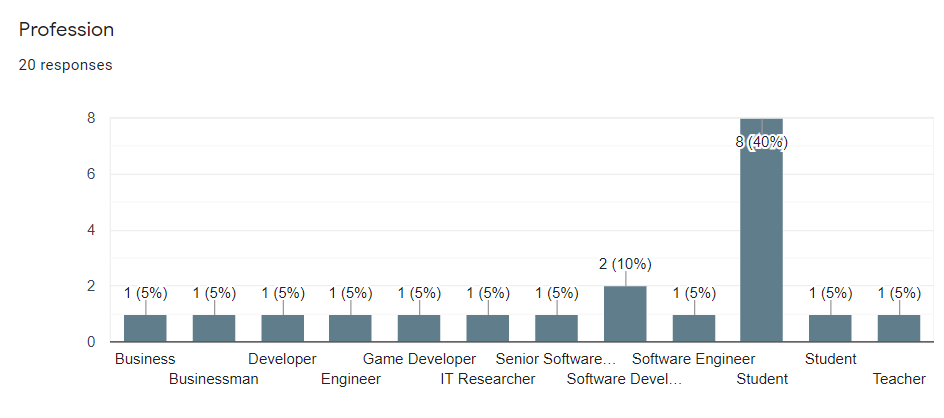
\includegraphics[width=0.9\textwidth]{img/Profession_Graph.PNG}
    \caption{Profession related details of participants}
    \label{fig:profGraph}
\end{figure}

\section{Conducted Surveys}
All participants were asked to complete two surveys. One named as "Frankenbot's Experience Survey" was designed with the help of \cite{MOLLER200726}\cite{itut}. For the second survey, the standardized tool to personally evaluate the usability and design of an interactive product known as AttrakDiff\cite{attrakdiff} has been used. First survey was designed using Google Forms and the purpose of it was to capture the user's interaction experience about the Frankenbot. While, the purpose of AttrakDiff's study was to evaluate different aspects such as Frankenbot's utility and usability. Furthermore, it also helped to weigh the chatbot for task-oriented and self-oriented qualities. 
\\~\\
The users were provided with the link to the deployed chatbot's interface as a web page and they can easily access it from their own places. It provided ease to the user and enhanced the comfortability factor for them. Also, they have to read the description and instructions provided for them on the web page. And they have to figure out what to do and how to operate the chatbot on their own without any external help. Which has given more realistic and unbiased essence to the results obtained.
\\~\\
For the surveys, the web page contains the heading as "Frankenbot's Request" in which the users were requested to complete the surveys once, they are finished having chat for a fun purpose with the chatbot. They have been provided with the links to both surveys.
\\~\\
The surveys were conducted in English language. Whereas, AttrakDiff's survey has the option for both English and German. You can find the "Frankenbot's Experience Survey" in the Appendices \ref{appen:survey}. Furthermore, AttrakDiff's Single Evaluation Study\cite{indeval} has been used as the second survey.
\\~\\
The questionnaires were filled by the participants on their own devices. As link to the deployed chatbot has been shared with them using different social platforms along with an introductory text about the purpose of the study. When the user was interacting with the chatbot all communication was getting stored in the log file for the future records and usage.

\section{Experimental Setup}
This research study has been conducted to gather the results for what user has experienced while interacting with the chatbot. The whole experiment itself has been divided in to four major parts mentioned below:
\begin{enumerate}
    \item Explanation of the chatbot for the participants in order to make its testing successful.
    \item Participants were requested for accomplishing set of tasks with the chatbot.
    \item The questionnaire to collect the user's interaction experience about the chatbot named as "Frankenbot's Experience Survey".
    \item Quality evaluation of the chatbot via AttrakDiff's Single Evaluation.
\end{enumerate} 
All of these are explained underneath in detail.

\subsection{Explanation of the Chatbot}
Users were provided with the description and instructions on the web page about the chatbot. The following sub-sections contain the required information and directions to for the users to operate the chatbot. Visual representation has been displayed in the Figure \ref{fig:userInter}.

\subsubsection*{Information}
The participants were provided with the introduction about the Frankenbot that it is the detective chatbot designed to interrogate you about the armed robbery happened few days back at a spatkauf near Berliner Strasse. It is responsible for investigating, so it is going to ask you some questions to come up with a decision. It will include, what it has investigated so far. Also you can have general conversation with it like you can ask it to talk about general stuff with you, about corona virus and its stats, to make you laugh, to do gossips, how does it feel, who is it, what does it eat and other related questions about the chatbot. You can switch between the topics at any moment as it is designed for parallel handling of the multiple topics. Kindly, communicate with it until it reaches any decision or says you goodbye before you jump to completion of the surveys.
\\~\\
Lastly, the ending of the information provided a brief note about how to re-initiate the chat. If user gets lost in between the dialogue and want to reinstate the detective game then just send a greeting message (hi, hello etc.) and the chatbot will restart it for him/her.

\subsubsection*{Instructions}
The user was asked to think as he/she is accused of a robbery and sitting in front of a detective and have to answer his brutal and tricky questions in order to prove his/her innocence. Otherwise, he/she will be declared as a culprit. It is a responsibility of a detective to make a decision based on user's answers to his questions.
\\~\\
At the end of the instructions there was a small notice available for the user to remove his/her doubts about its reality that it is the fictional detective chat bot designed only for testing and fun purpose.

\subsection{Tasks}
The participants were requested to accomplish following tasks beforehand, to fill the surveys.
\begin{itemize}
    \item Users were requested to play a small game with the detective chatbot and answer the questions, the way they wanted.
    \item They were also requested to have general dialogue with the chatbot. Ask it to talk about general stuff, about corona virus and its stats, to tell a joke, to do gossips, queries about its feelings and emotions and other related questions.
    \item Additionally, they were also asked to switch the topics. Means, they should start talking about general stuff if they are talking to the detective bot and vice versa by just replying to the last question of the previous topic.
    \item Lastly, they were requested not to leave the conversation in between until they reach the ending of the detective game. 
\end{itemize} 
\\~\\
All users were requested to chat with the chatbot at minimum, until it came up with any decision or says them goodbye. Other than that, there was no time restriction for them and they could have a dialogue for as long as they desired to.

\subsubsection*{Frankenbot's Request}
Finally, the user was requested that once he/she has finished having fun with the chatbot, please don't forget to complete two of the assessments provided as the links. The links were disabled when the web page gets loaded and gets activated after 1 minute, so that in meanwhile the user should get familiar with the chatbot by doing some chat with it. Frankenbot also stated that it welcomes and highly appreciates your prestigious feedback which will help its developer to get it evaluated and enhance its abilities for your better experience.

\subsection{Frankenbot's Experience Survey}
When the user successfully completed the tasks allocated to him/her. Then he/she filled out the survey about his/her interaction with the chatbot. The questionnaire itself has been divided in to the following sections:
\begin{itemize}
    \item Users overall impression about the interaction with the chatbot.
    \item Familiarity of the user with the already existing chatbots.
    \item Whether the user succeeded to achieve the desired goals.
    \item How was the communication with the chatbot.
    \item What was the behaviour of the chatbot with the users.
    \item How well the dialogue was designed.
    \item Personal impression and experience of the user about the chatbot.
    \item Users opinion about the chatbot's usefulness and user friendliness. 
\end{itemize} 
All sections have been consisted of several questions. And user has to respond by selecting an option out of linear scale from 1 to 5 whether he/she strongly agrees, agrees, undecided, disagrees or strongly disagrees with it. Most of the questions needed to be answered using these five options. Other than that overall impression about the chatbot has been measured using the linear scale of 5 options starting from 1 and ending on 5 as excellent, good, fair, poor and bad.

\subsubsection*{Overall Impression}
This section included a question about the user's overall impression about the interaction with the chatbot. It has been measured using the linear scale of 5 options starting from 1 and ending on 5 as excellent, good, fair, poor and bad. And out of the total 20 responses collected by the conduction of the survey, 2(10\%) responded with excellent mark and 9(45\%) rated it as good. So, total 11 out of 20 which is 55\% of the total participants, have passed positive remarks about it. Whereas, other 4(20\%) judged it as fair which also lies under the category of acceptable. So after summing up the percentages, 75\% of the participants rated their interaction as charming. On contrary, out of the remaining participants 3(15\%) rated it as poor and only 2(10\%) assigned it a bad label. So, it depicts that overall users impression about the interaction with the chatbot went well. For graphical representation of it, refer to the Figure \ref{fig:overallImpre}.

\begin{figure}[!h]
    \centering
    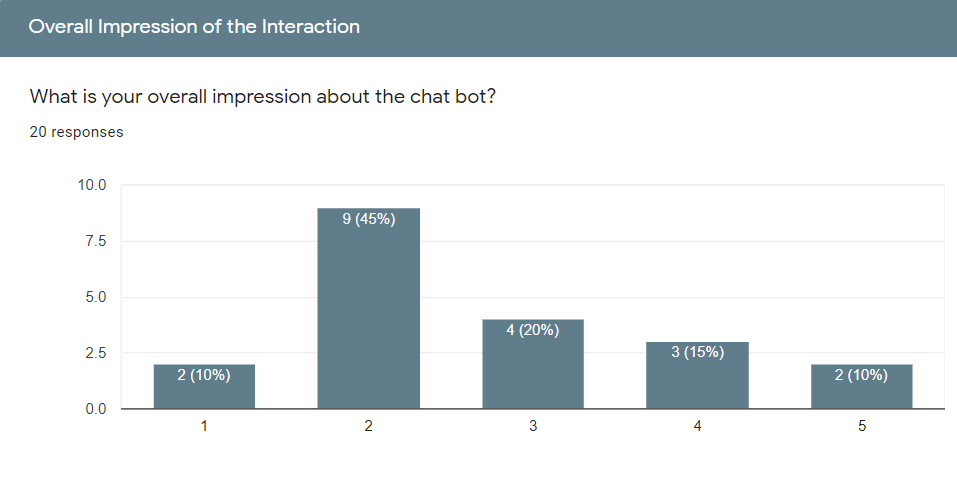
\includegraphics[width=0.9\textwidth]{img/Overall_Impression.PNG}
    \caption{Overall impression of the interaction with the chatbot}
    \label{fig:overallImpre}
\end{figure}

\subsubsection*{Familiarity with Existing Chat Bots}
This section added to the questionnaire just to figure out the experience of the participants with already existing chatbots that whether they are well familiar with the chatbots or are inexperienced with this emerging technology. So that, if majority of them have the good knowledge of any of the existing chatbots, it will provide more strength and solidity to the results gathered from such participants.
\\~\\
There were total 3 questions available under this section that participants have to answer:
\begin{enumerate}
    \item I feel that I am well familiar with the chat bots like Google Assistant, Apple's Siri etc. (Possible options lie between scale of strongly agree to strongly disagree).
    \item I communicate with the chat bots. And the possible options provided were Frequently (daily or several times in a week), Seldomly (rarely in weeks or months), Just few times and Never.
    \item Purpose of my chat bots usage is: (only if you answered question no. 2 positively). Possible answers could be any out of the followings: Personal commands to provide you assistance in performing tasks, For fun, Not feel lonely and No reason.
\end{enumerate}
Fortunately, for the first statement, 16(80\%) appeared to be well familiar with the existing chatbots. 2(10\%) answered with undecided and remaining 2(10\%) just disagreed with the statement but no one strongly disagreed with it. Graph depicting such results has been shown in the Figure \ref{fig:familiarity}. Coming to the second statement, 5(25\%) detected to be frequent users. 8(40\%) resulted to be the seldom users. Whereas, 6(30\%) communicated just few times with the chatbots as shown in the Figure \ref{fig:commChatRes}. Lastly, almost 60\% knew how to operate and give commands to the chatbot. And around 30\% appeared to use it for joy and fun purpose. These all stats and readings portrays that experienced users participated in this study. And results obtained from the study is trustworthy and reliable. 

\begin{figure}[!h]
    \centering
    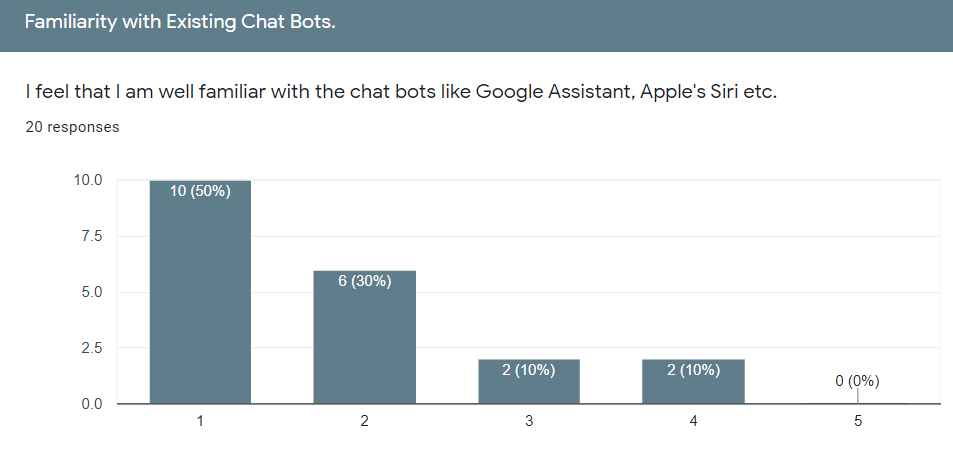
\includegraphics[width=0.9\textwidth]{img/Familiraity.PNG}
    \caption{Participants familiarity with the chat bots like Google Assistant, Apple's Siri etc.}
    \label{fig:familiarity}
\end{figure}

\begin{figure}[!h]
    \centering
    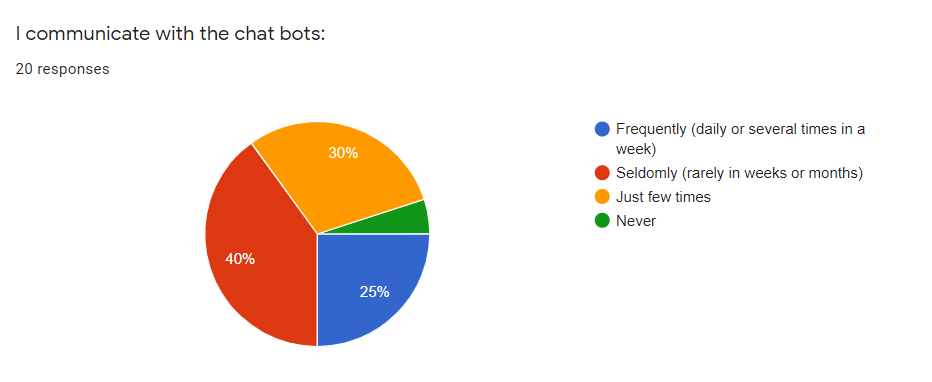
\includegraphics[width=0.9\textwidth]{img/Communicate_Chatbots_Result.PNG}
    \caption{Participants usage of the chat bots like Google Assistant, Apple's Siri etc.}
    \label{fig:commChatRes}
\end{figure}

\subsubsection*{Achievement of Goals}
It highlights whether the user succeeded to achieve the desired goals or not while having an interaction with the chatbot. It contains the following questions in respond to which user checked an option, including or in between of strongly agree to strongly disagree.
\begin{enumerate}
    \item The information provided by the chat bot was clear.
    \item The provided information was incomplete.
    \item The interaction with the chat bot was efficient.
    \item The chat bot is unreliable.
\end{enumerate}
Discussing the results and stats for the very first statement, 13(65\%) participants agreed upon the information provided by the chatbot was clear. Whereas, 3(15\%) were failed to decide about it. Only 4(20\%) just disagreed with it and no one strongly negated it. For better understanding of it just see the Figure \ref{fig:clearInfo}.

\begin{figure}[!h]
    \centering
    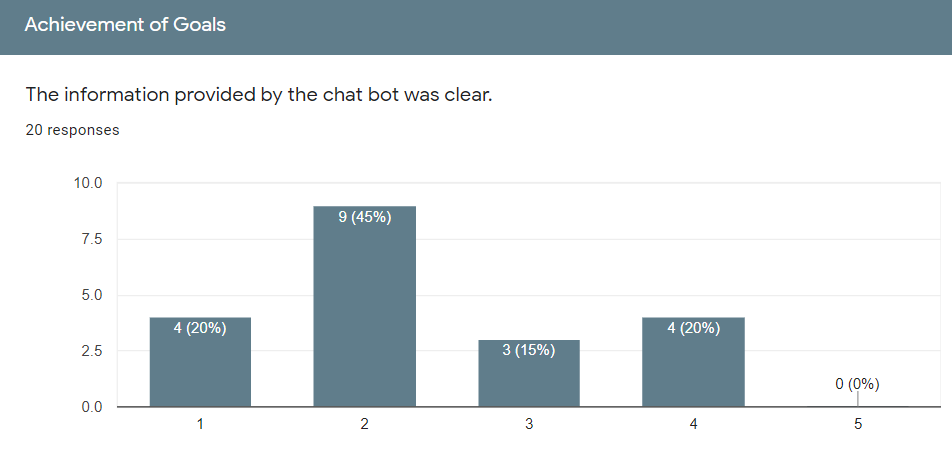
\includegraphics[width=0.9\textwidth]{img/Clear_Info.PNG}
    \caption{Stats depicting about the information provided by the chat bot was clear}
    \label{fig:clearInfo}
\end{figure}
\\~\\
For the second statement, 10(50\%) disagreed with it which tells that for them the provided information was complete. Whilst 7(35\%) were unable to make any decision about it. This is something can not ignored. It can happen due to various reasons: (i) due to lack of concentration (ii) misinterpretation of information or instructions (iii) chatbot responded falsely and the only reason for it could be a weakly trained Rasa's NLU due to limited training data. But still 50\% answered that the information was complete, so there are high chances that the reason lies somewhere between (i) and (ii). Visuals have been shown in the Figure \ref{fig:incompInfo}.

\begin{figure}[!h]
    \centering
    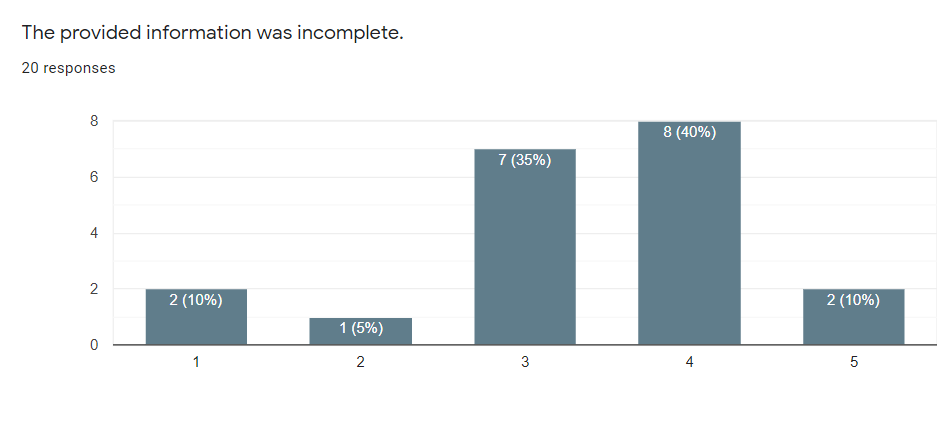
\includegraphics[width=0.9\textwidth]{img/Incomp_Info.PNG}
    \caption{Stats depicting about the provided information was incomplete}
    \label{fig:incompInfo}
\end{figure}
\\~\\
Moving to what has been concluded from the third statement seems to be something really positive. As 12(60\%) of the participants agreed upon the efficient interaction with the chatbot. Moreover, 4(20\%) failed to decide about it and only other remaining 4(20\%) disagreed with it. Refer to the Figure \ref{fig:effInt} for seeing the detailed graph of it.

\begin{figure}[!h]
    \centering
    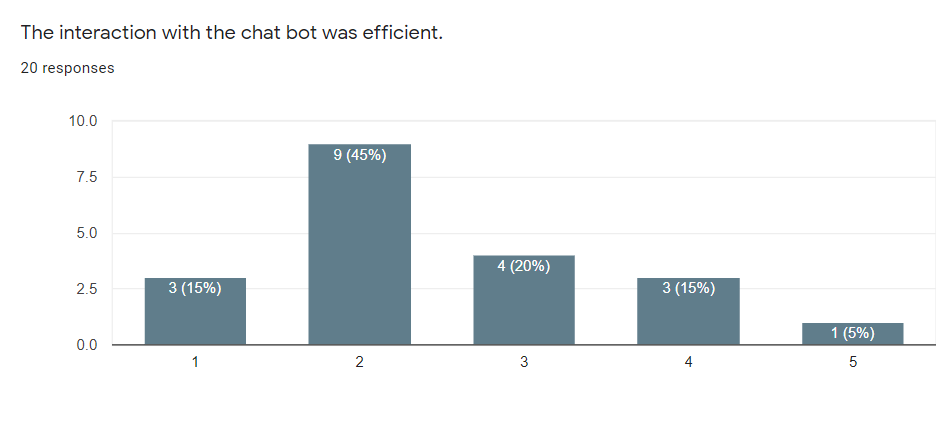
\includegraphics[width=0.9\textwidth]{img/Efficient_Inter.PNG}
    \caption{Stats depicting about the interaction with the chat bot was efficient}
    \label{fig:effInt}
\end{figure}
\\~\\
Lastly, forth statement stats are a bit disappointing. According to only 6(30\%) users, the chatbot was reliable. On contrary, 8(40\%) declared it unreliable and remaining 6(30\%) failed to take any decision about it. The possible reason for its unreliability could be its inability to respond the user for all of his/her queries. And it is happening due to limited data provided for training and also the demo chatbot was designed for limited use cases. In order to design a fully loaded chatbot that can reply to the user for any of his/her utterance, lot of training data and processing is required and within limited time and resources it was not possible. But, it could be done in future. See the Figure \ref{fig:unreliBot} for better understanding of results.

\begin{figure}[!h]
    \centering
    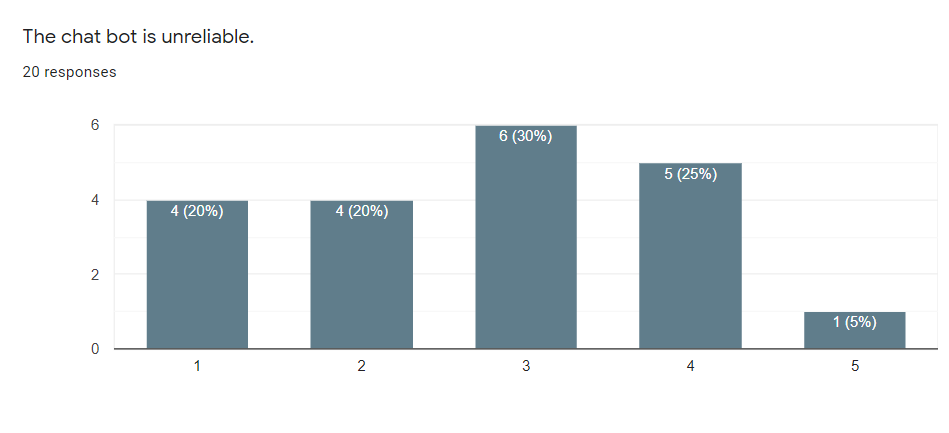
\includegraphics[width=0.9\textwidth]{img/Unreli_Bot.PNG}
    \caption{Stats depicting about the chat bot is unreliable}
    \label{fig:unreliBot}
\end{figure}

\subsection{Evaluation via AttrakDiff}
The tool's single evaluation method has been used in order to judge the chatbot on the basis  of the following qualities:
\begin{itemize}
    \item Hedonic quality (joy of use, emphasized stimulation, identification and evocation generated by the system).
    \item Pragmatic quality (usefulness, efficiency, easy to use).
\end{itemize} 


